\documentclass[ijoo,nonblindrev]{informs-ijoo}

\OneAndAHalfSpacedXI
%%\OneAndAHalfSpacedXII % Current default line spacing
%%\DoubleSpacedXII
%%\DoubleSpacedXI

% Private macros here (check that there is no clash with the style)

% Natbib setup for author-year style
\usepackage{natbib}
\bibpunct[, ]{(}{)}{,}{a}{}{,}%
\def\bibfont{\small}%
\def\bibsep{\smallskipamount}%
\def\bibhang{24pt}%
\def\newblock{\ }%
\def\BIBand{and}%

%% Setup of theorem styles. Outcomment only one.
%% Preferred default is the first option.
\TheoremsNumberedThrough     % Preferred (Theorem 1, Lemma 1, Theorem 2)
%\TheoremsNumberedByChapter  % (Theorem 1.1, Lema 1.1, Theorem 1.2)
\ECRepeatTheorems

%% Setup of the equation numbering system. Outcomment only one.
%% Preferred default is the first option.
\EquationsNumberedThrough    % Default: (1), (2), ...
%\EquationsNumberedBySection % (1.1), (1.2), ...

% For new submissions, leave this number blank.
% For revisions, input the manuscript number assigned by the on-line
% system along with a suffix ".Rx" where x is the revision number.
\MANUSCRIPTNO{MS-0001-1922.65}

\usepackage{amssymb,amsmath,amsfonts}
\usepackage{latexsym}
\usepackage{graphicx}
\usepackage{mathrsfs}
\usepackage{fancyhdr}
\usepackage{booktabs}
\usepackage{color}
\usepackage[english]{babel}
\usepackage[utf8]{inputenc}
\usepackage{algorithm, algorithmicx, algpseudocode}
\usepackage{authblk}
%\usepackage[width=17.00cm, height=25.00cm]{geometry}
\usepackage{multirow}

%\usepackage{tikz}
%\usetikzlibrary{backgrounds,fit, arrows}
%
%\usepackage{natbib}
%\bibpunct[, ]{(}{)}{,}{a}{}{,}%
%\def\bibfont{\small}%
%\def\bibsep{\smallskipamount}%
%\def\bibhang{24pt}%
%\def\newblock{\ }%
%\def\BIBand{and}%

%\newtheorem{theorem}{\sffamily Theorem}
%\newtheorem{axiom}{\sffamily Axiom}
%\newtheorem{case}{\sffamily Case}
%\newtheorem{claim}{\sffamily Claim}
%\newtheorem{conclusion}{\sffamily Conclusion}
%\newtheorem{condition}{\sffamily Condition}
%\newtheorem{conjecture}{\sffamily Conjecture}
%\newtheorem{corollary}{\sffamily Corollary}
%\newtheorem{criterion}{\sffamily Criterion}
%\newtheorem{definition}{\sffamily Definition}
%\newtheorem{example}{\sffamily Example}
%\newtheorem{exercise}{\sffamily Exercise}
%\newtheorem{lemma}{\sffamily Lemma}
%\newtheorem{notation}{\sffamily Notation}
%\newtheorem{problem}{\sffamily Problem}
%\newtheorem{proposition}{\sffamily Proposition}
%\newtheorem{remark}{\sffamily Remark}
%\newtheorem{solution}{\sffamily Solution}
%\newtheorem{summary}{\sffamily Summary}
%\newtheorem{assumption}{\sffamily Assumption}

%%%%%%%%%%%%%%%%
\begin{document}
	%%%%%%%%%%%%%%%%
	
	% Outcomment only when entries are known. Otherwise leave as is and
	%   default values will be used.
	%\setcounter{page}{1}
	%\VOLUME{00}%
	%\NO{0}%
	%\MONTH{Xxxxx}% (month or a similar seasonal id)
	%\YEAR{0000}% e.g., 2005
	%\FIRSTPAGE{000}%
	%\LASTPAGE{000}%
	%\SHORTYEAR{00}% shortened year (two-digit)
	%\ISSUE{0000} %
	%\LONGFIRSTPAGE{0001} %
	%\DOI{10.1287/xxxx.0000.0000}%
	
	% Author's names for the running heads
	% Sample depending on the number of authors;
	% \RUNAUTHOR{Jones}
	\RUNAUTHOR{Contardo}
	% \RUNAUTHOR{Jones, Miller, and Wilson}
	% \RUNAUTHOR{Jones et al.} % for four or more authors
	% Enter authors following the given pattern:
	%\RUNAUTHOR{}
	
	% Title or shortened title suitable for running heads. Sample:
	% \RUNTITLE{Bundling Information Goods of Decreasing Value}
	% Enter the (shortened) title:
	\RUNTITLE{Decremental clustering for the $p$-dispersion problem}
	
	% Full title. Sample:
	% \TITLE{Bundling Information Goods of Decreasing Value}
	% Enter the full title:
	\TITLE{Decremental clustering for the solution of $p$-dispersion problems to proven optimality}
	
	% Block of authors and their affiliations starts here:
	% NOTE: Authors with same affiliation, if the order of authors allows,
	%   should be entered in ONE field, separated by a comma.
	%   \EMAIL field can be repeated if more than one author
	\ARTICLEAUTHORS{%
		\AUTHOR{Claudio Contardo}
		\AFF{Department of management and technology, ESG UQAM, GERAD and CIRRELT \\\EMAIL{E-mail address: claudio.contardo@gerad.ca}} %, \URL{}}
%		\AUTHOR{Marg Arinella}
%		\AFF{Institute for Food Adulteration, University of Food Plains, Food Plains, MN 55599, \EMAIL{m.arinella@adult.ufp.edu}}
		% Enter all authors
	} % end of the block
	
	\ABSTRACT{%
		Given $n$ points, a symmetric dissimilarity matrix $D$ of dimensions $n\times n$ and an integer $p\geq 2$, the $p$-dispersion problem (\pDP{}) consists in selecting a subset of exactly $p$ points in such a way that the minimum dissimilarity between any pair of selected points is maximum. The \pDP{} is \nphard{} when $p$ is an input of the problem. We propose a decremental clustering method to reduce the problem to the solution of a series of smaller \pDP{}s until reaching proven optimality. The proposed method can handle problems orders of magnitude larger than the limits of the state-of-the-art solver for the \pDP{} for small values of $p$.
		% Enter your abstract
	}%
	
	% Sample
	%\KEYWORDS{deterministic inventory theory; infinite linear programming duality;
	%  existence of optimal policies; semi-Markov decision process; cyclic schedule}
	
	% Fill in data. If unknown, outcomment the field
	\KEYWORDS{decremental clustering, p-dispersion problem, exact algorithm.}
	\HISTORY{Submitted on \today.}
	
	%%%%%%%%%%%%%%%%%%%%%%%%%%%%%%%%%%%%%%%%%%%%%%%%%%%%%%%%%%%%%%%%%%%%%%
	
	% Samples of sectioning (and labeling) in MNSC
	% NOTE: (1) \section and \subsection do NOT end with a period
	%       (2) \subsubsection and lower need end punctuation
	%       (3) capitalization is as shown (title style).
	%
	%\section{Introduction.}\label{intro} %%1.
	%\subsection{Duality and the Classical EOQ Problem.}\label{class-EOQ} %% 1.1.
	%\subsection{Outline.}\label{outline1} %% 1.2.
	%\subsubsection{Cyclic Schedules for the General Deterministic SMDP.}
	%  \label{cyclic-schedules} %% 1.2.1
	%\section{Problem Description.}\label{problemdescription} %% 2.
	
	% Text of your paper here
% ################ IJOO TEMPLATE HEADER ENDS HERE

%\documentclass[a4paper,10pt]{article}

%%%%%%%%%%%%%%%%%%%%%%%%%%%%%%%%%%%%%%%%%%%%%%%%%%%
%%%%% Start of author commands %%%%%%%%%%%%%%%%%%%%
%%%%%%%%%%%%%%%%%%%%%%%%%%%%%%%%%%%%%%%%%%%%%%%%%%%
% Add your commands
\newcommand{\nphard}{$\mathcal{NP}$-hard}
\newcommand{\pDP}{\texttt{pDP}}
\newcommand{\pdp}[2]{$\mathtt{pDP({#1}, {#2})}$}
\newcommand{\cev}[1]{\reflectbox{\ensuremath{\vec{\reflectbox{\ensuremath{#1}}}}}}
\newcommand{\mC}{\mathcal{C}}
\newcommand{\DmC}{D^{\mC}}
\newcommand{\hpdp}[2]{$\mathtt{heuristicPDP({#1}, {#2})}$}
\newcommand{\initclust}[3]{$\mathtt{initialClustering({#1}, {#2}, {#3})}$}
\newcommand{\splitadd}[4]{$\mathtt{splitAndAdd({#1}, {#2}, {#3}, {#4})}$}
\newcommand{\buildDmC}[1]{$\mathtt{buildReducedDissMat({#1})}$}
\newcommand{\solvePDP}[2]{$\mathtt{solvePDP({#1}, {#2})}$}
\newcommand{\exactPDP}[4]{$\mathtt{exactPDP({#1}, {#2}, {#3}, {#4})}$}
%%%%%%%%%%%%%%%%%%%%%%%%%%%%%%%%%%%%%%%%%%%%%%%%%%%
%%%%% End of author commands %%%%%%%%%%%%%%%%%%%%%%
%%%%%%%%%%%%%%%%%%%%%%%%%%%%%%%%%%%%%%%%%%%%%%%%%%%


%%%%%%%%%%%%%%%%%%%%%%%%%%%%%%%%%%%%%%%%%%%%%%%%%%%
%%%%% Begin Document - DO NOT TOUCH %%%%%%%%%%%%%%%
%%%%%%%%%%%%%%%%%%%%%%%%%%%%%%%%%%%%%%%%%%%%%%%%%%%

%\begin{document}

%%%%%%%%%%%%%%%%%%%%%%%%%%%%%%%%%%%%%%%%%%%%%%%%%%%
%%%%% Title, authors, contact info **FILL OUT** %%%
%%%%%%%%%%%%%%%%%%%%%%%%%%%%%%%%%%%%%%%%%%%%%%%%%%%
%\title{Decremental clustering for the exact solution of some large-scale $p$-dispersion problems}
%\author[ ]{Claudio Contardo}
%\affil[ ]{Department of management and technology, ESG UQAM, GERAD and CIRRELT}
%\affil[ ]{e-mail address: claudio.contardo@gerad.ca}

%\maketitle

%\begin{abstract}
%
%\end{abstract}
\maketitle

%%%%%%%%%%%%%%%%%%%%%%%%%%%%%%%%%%%%%%%%%%%%%%%
\section{Introduction\label{section:intro}}

In the $p$-dispersion problem (\pDP{}) we are given a set of $n$ points, a symmetric dissmilarity matrix $D = \{D(i, j): 1\leq i, j\leq n\}$ satisfying $D(i, j) \geq 0$ for every $1\leq i, j\leq n$ and $D(i, i) = 0$ for every $1\leq i\leq n$, and an integer $p\geq 2$. The objective is to select $p$ points from the set of $n$ so as to maximize the minimum pairwise dissimilarity within the selected points. The \pDP{}, as noticed by \citet{Erkut1990discrete}, is \nphard{} when $p$ makes part of the input parameters (otherwise it can be solved in $O(n^p)$ time by exhaustive enumeration). We denote this problem, for given input parameters $D$ and $p$ ($n$ is implicitly given in the dimensions of $D$), as \pdp{D}{p}.%$\mathtt{pDP(D, p)}$. 

The \pDP{} arises in a number of practical contexts. In location analysis, a \pDP{} can help decide the placement of installations whose proximity may be hazardous ---as is the case of power plants, oil storage tanks or ammunition---, or in the location of retail stores to prevent cannibalization \citep{Kuby1987Programming}. In multiobjective optimization, in the presence of multiple solutions for a given optimization problem, one may solve a \pDP{} to select a subset of those solutions as complementary as possible with respect to the values for each of the objectives \citep{Saboonchi2014MaxMinMin}. In finance, a \pDP{} can be used as a proxy to build diversified portfolios, which are known to provide low risk \citep{Statman1987how}.
	
The state-of-the-art solver for the \pDP{} \citep{Sayah2017new} relies on the solution of an integer program containing $O(n + \Delta)$ variables and constraints, where $\Delta$ is the number of distinct entries in the dissimilarity matrix $D$. The model remains tractable for medium-sized problems but memory/time limits may prevent the solution of problems containing more than a few hundred nodes. The problem size and the large amount of symmetries impact the model's performance. 

Our article contributes at narrowing this gap by allowing the solution of potentially much larger problems (in terms of the number of nodes $n$), under the assumption that parameter $p$ remains low (typically $\leq 10$ when going large-scale). To this end, we introduce a decremental clustering scheme that in a dynamic fashion forms clusters of points and constructs instances of the \pDP{} that are smaller in size and with much better numerical properties (most notably a much smaller amount of symmetries). These smaller instances are shown to provide upper bounds of the original problem and are much more tractable than the original \pDP{}. The proposed iterative mechanism can scale and solve problems containing up to 100,000 nodes to proven optimality within reasonable time limits, this is orders of magnitude larger than the scope of previous methods. While clustering techniques are of common use in the development of metaheuristics, this is to the best of our knowledge the first time that they are embedded within an exact solver for combinatorial optimization problems arising in location analysis.

The remainder of this article is organized as follows. In Section \ref{section:litreview} we present a review of the relevant scientific literature related to this article. In Section \ref{section:decrclust} we present the decremental clustering framework. In Section \ref{section:computation} we present the results of our computational campaign to assess the effectiveness of our method. Finally, Section \ref{section:conclusions} concludes the paper.

\section{Literature review\label{section:litreview}}

Applications of the \pDP{} can be found in multiple fields including location analysis, multiobjective optimization and portfolio optimization. \citet{Kuby1987Programming} mention the importance of locating facilites are far as possible from each other when they represent a potential hazard for the surrounding communities. The same authors also mention applications in store location. If two stores of the same chain are located too close, cannibalism may prevent them from selling at full potential. \citet{Saboonchi2014MaxMinMin} discuss an application of the \pDP{} in multiobjective optimization. If the Pareto frontier of a problem contains multiple solutions, one shall solve a \pDP{} to find $p$ such solutions with distinct features. The same authors also describe an application in portfolio optimization to ---given a set of potential investment opportunities--- choose a subset that reduces the closeness in terms of features between the different investment options so as to reduce the risk associated with the portfolio. The problem of selecting diversified portfolios has been recognized as of most importance in Finance \citep{Statman1987how}.

The \pDP{} is tightly related to facility location problems (FLP, \citet{Laporte2015Location}). In its simplest version, a FLP corresponds to the problem of, given a set of potential facility locations and a set of customers, select a subset of potential facility locations and allocate the customers to those facilities, at minimum total cost. Facility location problems and applications have been widely studied in the scientific literature, and several comprehensive surveys have been recently published that take into account several of the latest advances in the field \citep{Laporte2015Location, Melo2009Facility}. The \pDP{} differs from a typical FLP model in the importance of the notion of customer. While they are of key importance for the right choice of the facilities in the FLP, in the \pDP{} they are irrelevant. Only the facility locations are of importance, and their choice must reflect the objective function to be optimized: to maximize the minimum distance between any two chosen facilities. One particular variant of FLP, namely the obnoxious $p$-median problem (OpMP, \citet{Belotti2006branch}), is closely related fo the \pDP{}. In the OpMP, we are given a set of potential facilities and of customers. A planner must select the location of $p$ facilities in such a way that the minimum distance from any customer to its closest facility is maximized. This problem arises in the location of hazardous or obnoxious installations.

The \pDP{} is also related to clustering problems, and more specifically to the maximin split clustering problem (MMSCP). In the MMSCP, we are given a set $N$ of observations, a dissmilarity matrix $D$ and a target number of clusters $p$. One has to group the observations into $p$ groups such that the minimum dissimilarity between any two observations belonging to different groups is maximized. The MMSCP, unlike the \pDP{}, is polynomially solvable \citep{Delattre1980Bicriterion}.

Regarding the methodological contributions to the solution of the \pDP{}, a handful of articles have dealt with the problem of solving the \pDP{} to proven optimality. \citet{Pisinger2006Upper} introduces a quadratic formulation for the \pDP{} which is then partially solved by a series of relaxations including semidefinite programming, and linearization-reformulation. The bounds are embedded within a branch-and-bound framework and the author reports the solution of problems containing a few hundred nodes. \citet{Kuby1987Programming} introduces a mixed-integer linear formulation of the problem with a series of Big-M coefficients. The model can be seen as a linearization of that of \citet{Pisinger2006Upper} even though it was introduced almost 20 years earlier. The model is more compact than that of \citet{Pisinger2006Upper} but provides much weaker upper bounds. \citet{Sayah2017new} introduces a novel pure binary compact formulation of the problem that the authors solve by branch-and-cut. Clique-like inequalities are used to strengthen the model. Problems with up to 1,000 nodes are solved to proven optimality as reported by the authors. The same authors also mention that linear and binary search methods may be used with the different formulations to speed up the solution process. Such techniques have already been studied by \citet{Chandrasekaran1981Location, Pisinger2006Upper} for the \pDP{}. For this to be beneficial, the models need to exploit the availability of lower and upper bounds to fathom non-promising branches of the implicit enumeration tree.

The decremental clustering method introduced in this article is tightly related to other decremental relaxation mechanisms recently introduced in the literature for the solution of other MiniMax (or equivalently MaxiMin) combinatorial optimization problems to proven optimality. In the vertex p-center problem (VPCP), for the same input parameters $n, D$ and $p$, one has to select $p$ points and allocate the remaining points to their closest centers in such a way that the maximum dissimilarity between a node and its assigned center is minimized. \citet{Chen2009New} and \citet{Contardo2019scalable} propose decremental relaxation mechanisms to ignore some node allocation constraints, which are only added as needed. The relaxed problems can thus be modeled as smaller VPCPs in an iterative manner. \citet{Contardo2019scalable} report the solution of problems containing up to 1M observations to proven optimality. The minimax diameter clustering problem (MMDCP) is another problem for which the decremental relaxation mechanism has proven useful. In the MMDCP, given $n$ points, a dissmilarity matrix $D$ and an integer $k\geq 2$, the objective is to group the observations into $k$ clusters such as to minimize the maximum intra-cluster dissimlarity. \citet{Aloise2018sampling} introduced a sampling mechanism to solve the MMDCP as a series of smaller MMDCPs in a dynamic fashion, allowing the solution to proven optimality of problems containing up to 600k observations.

Using clustering mechanisms for finding feasible solutions for hard combinatorial optimization problems is not something totally new in the operations research literature. Embedding a clustering scheme within a heuristic solver has been common practice for many years and for multiple classes of problems. In vehicle routing and scheduling, the so-called cluster-first-route-second \citep{Solomon1987algorithms, Braysy2005Vehicle} and route-first-cluster-second \citep{Beasley1983route, Prins2014Order} paradigms are both based on combining routing and clustering techniques so as to reduce the computational burden associated with the routing or scheduling substructures. None of those techniques, however, provide any guarantee of optimality.

\section{Decremental clustering\label{section:decrclust}}

In this section we describe the decremental clustering method for the \pDP{}. This section is subdivided in 5 subsections. In the first subsection, we provide the theoretical foundations and a high-level description of the method. The next four sections describe the different procedures of the method.

\subsection{High-level description and theoretical foundations}

Let us introduce some notation and vocabulary first. A \textit{clustering} of the $n$ nodes, and denoted by $\mC$, is a family $\{C_i: i = 1 \ldots m\}$ such that (i) $C_i\cap C_j =\emptyset$ for every $1\leq i < j\leq m$ and (ii) $\bigcup\{C_i: i=1\ldots m\} = \{1\ldots n\}$ . A clustering $\mC$ is said to be \textit{sufficiently refined} if, for every set $C_i\in\mathcal{C}$, $D(C_i) := \max\{D(u, v): u, v\in C_i, u < v\} < z^*$, where $z^*$ is the optimal value of problem \pdp{D}{p}. For practical purposes, it is sufficient to test the refinement of a clustering with respect to a lower bound $l \leq z^*$. The correctness of the decremental clustering method is supported on the following result.

\begin{lemma}\label{proposition:lemma1}
	Let $\mC$ be a sufficiently refined clustering of the nodes of size $m$. Let $\DmC$ be a $m\times m$ dissimilarity matrix where $\DmC(i, j) = \max\{D(u, v): u\in C_i, v\in C_j\}$. The optimal value $\zeta^*$ of the problem \pdp{\DmC}{p} provides an upper bound of problem \pdp{D}{p}.
\end{lemma}
\proof{Proof of Lemma \ref{proposition:lemma1}}
	Let $S = \{s_1\ldots s_p\}$ be an optimal solution of problem \pdp{D}{p}, of value $z^*$. Because the clustering $\mC$ is sufficiently refined, it follows that no two nodes in $S$ can be found in the same cluster $C\in\mC$. For every $s\in S$, let $k(s)$ denote the cluster index in $\mC$ where node $s$ lies. By construction of $\DmC$, we have that $D(s, t)\leq \DmC(k(s), k(t))$ for every two nodes $s, t\in S, s < t$ and therefore $z^* \leq \zeta^*$.\Halmos
\endproof

Our method works as follows. First, a lower bound $L \leq z^*$ is computed using a simple heuristic (using procedure \hpdp{D}{p}, see Section \ref{section:decrclust:hpdp}). An initial upper bound $U$ is also computed as simply the largest dissimlarity between any two points in the dataset. Using the lower bound $L$, we build an initial sufficiently refined clustering $\mC$ and a reduced dissmilarity matrix $\DmC$ (using procedure \initclust{D}{p}{L}, see Section \ref{section:decrclust:initclust}). We initially let $S, W\leftarrow\emptyset$, where $S$ represents the set of optimal non-singleton clusters, and $W$ the complete optimal solution to the restricted \pDP{}. In an iterative fashion, we use the sets $S, W$ to refine the current clustering, yielding a refined clustering $\mC$ and dissimilarity matrix $\DmC$ (using procedure \splitadd{S}{W}{\mC}{\DmC}, see Section \ref{section:decrclust:splitadd}). The resulting reduced \pDP{} is then solved yielding an upper bound $U$ and its optimal solution is used to update the sets $S, W$ (using procedure \solvePDP{\DmC}{p}, see Section \ref{section:decrclust:solvepdp}), after which the algorithm iterates. The pseudo-code provided in 
Algorithm \ref{alg:decrclust} formalizes the main steps of our algorithm.% The detail of the different subprocedures used is given in the following subsections.

\begin{algorithm}[H]
	\caption{Decremental clustering for \pdp{D}{p}\label{alg:decrclust}}
	\begin{algorithmic}\normalsize
		\Require $D, p$
		\Ensure Set $X = \{x_1\ldots x_p\}$ of optimal locations
		\State $L\leftarrow$\hpdp{D}{p}, $U\leftarrow\max\{D(i, j): 1\leq i < j \leq n\}$
		\State $\mC, \DmC\leftarrow$\initclust{D}{p}{L}
		\State $S\leftarrow\emptyset, W\leftarrow\emptyset$
		\Repeat
			\State $\mC, \DmC\leftarrow$\splitadd{S}{W}{\mC}{\DmC}
			\State $U, W\leftarrow$\solvePDP{\DmC}{p}%\Comment{$U\leftarrow$ optimal value, $X\leftarrow$ optimal solution}
			\State $S\leftarrow\{w\in W : |C_w| \geq 2\}$
		\Until{$S = \emptyset$}
		\State \textbf{return} $X\leftarrow\{C_w: w\in W\}$
	\end{algorithmic}
\end{algorithm}

The following proposition formalizes the exactness of the decremental clustering procedure.

\begin{proposition}\label{proposition:prop1}
	The decremental clustering method ends in at most $n$ iterations and produces an optimal solution to problem \pdp{D}{p}.
\end{proposition}
\proof{Proof of Proposition \ref{proposition:prop1}}
	Let $X = \{x_1\ldots x_p\}$ be the optimal solution of problem \pdp{\DmC}{p}. If the clusters corresponding to the solution $X$ are all singletons, then this is also a feasible solution to problem \pdp{D}{p} and therefore produces a lower bound that matches with the upper bound provided by problem \pdp{\DmC}{p}. Otherwise, the method identifies at least one cluster $i$ such that $|C_i| \geq 2$ and splits it into two separate groups. This can be done at most $n$ times when the clusters in $\mC$ become all singletons.\Halmos
\endproof

In Figure \ref{fig:mu1979} we illustrate by means of an example the result of applying the decremental clustering mechanism on instance \texttt{mu1979.tsp} from the TSPLIB for $p = 5$. In the left, we plot all the 1,979 data points of the dataset. In the right, we plot circles representing the different clusters at the last iteration of the method, which are only 47. This means that the largest reduced \pDP{} solved by our method contained 47 points and the associated dissimilarity matrix was of dimensions $47\times 47$, this is orders of magnitude smaller than the sizes of the original data structures. The extreme points of the edges appearing in the right represent the optimal solution of the problem, with the solid red line representing the optimal dissimilarity of 3,845. We would like to highlight the following key observation. Note the right-most point in the optimal solution to the problem surrounded by other points that may be even further from the other 4 points in the optimal solution. Therefore many of those points could be used to replace the one chosen by the algorithm yielding an equally good value. This is also true for the point in the bottom-left corner chosen by the algorithm. A careless handling of the dataset would result in a substantial amount of symmetries that our algorithm, however, avoids in a large amount.

\begin{figure}[!hbtp]
	\centering
	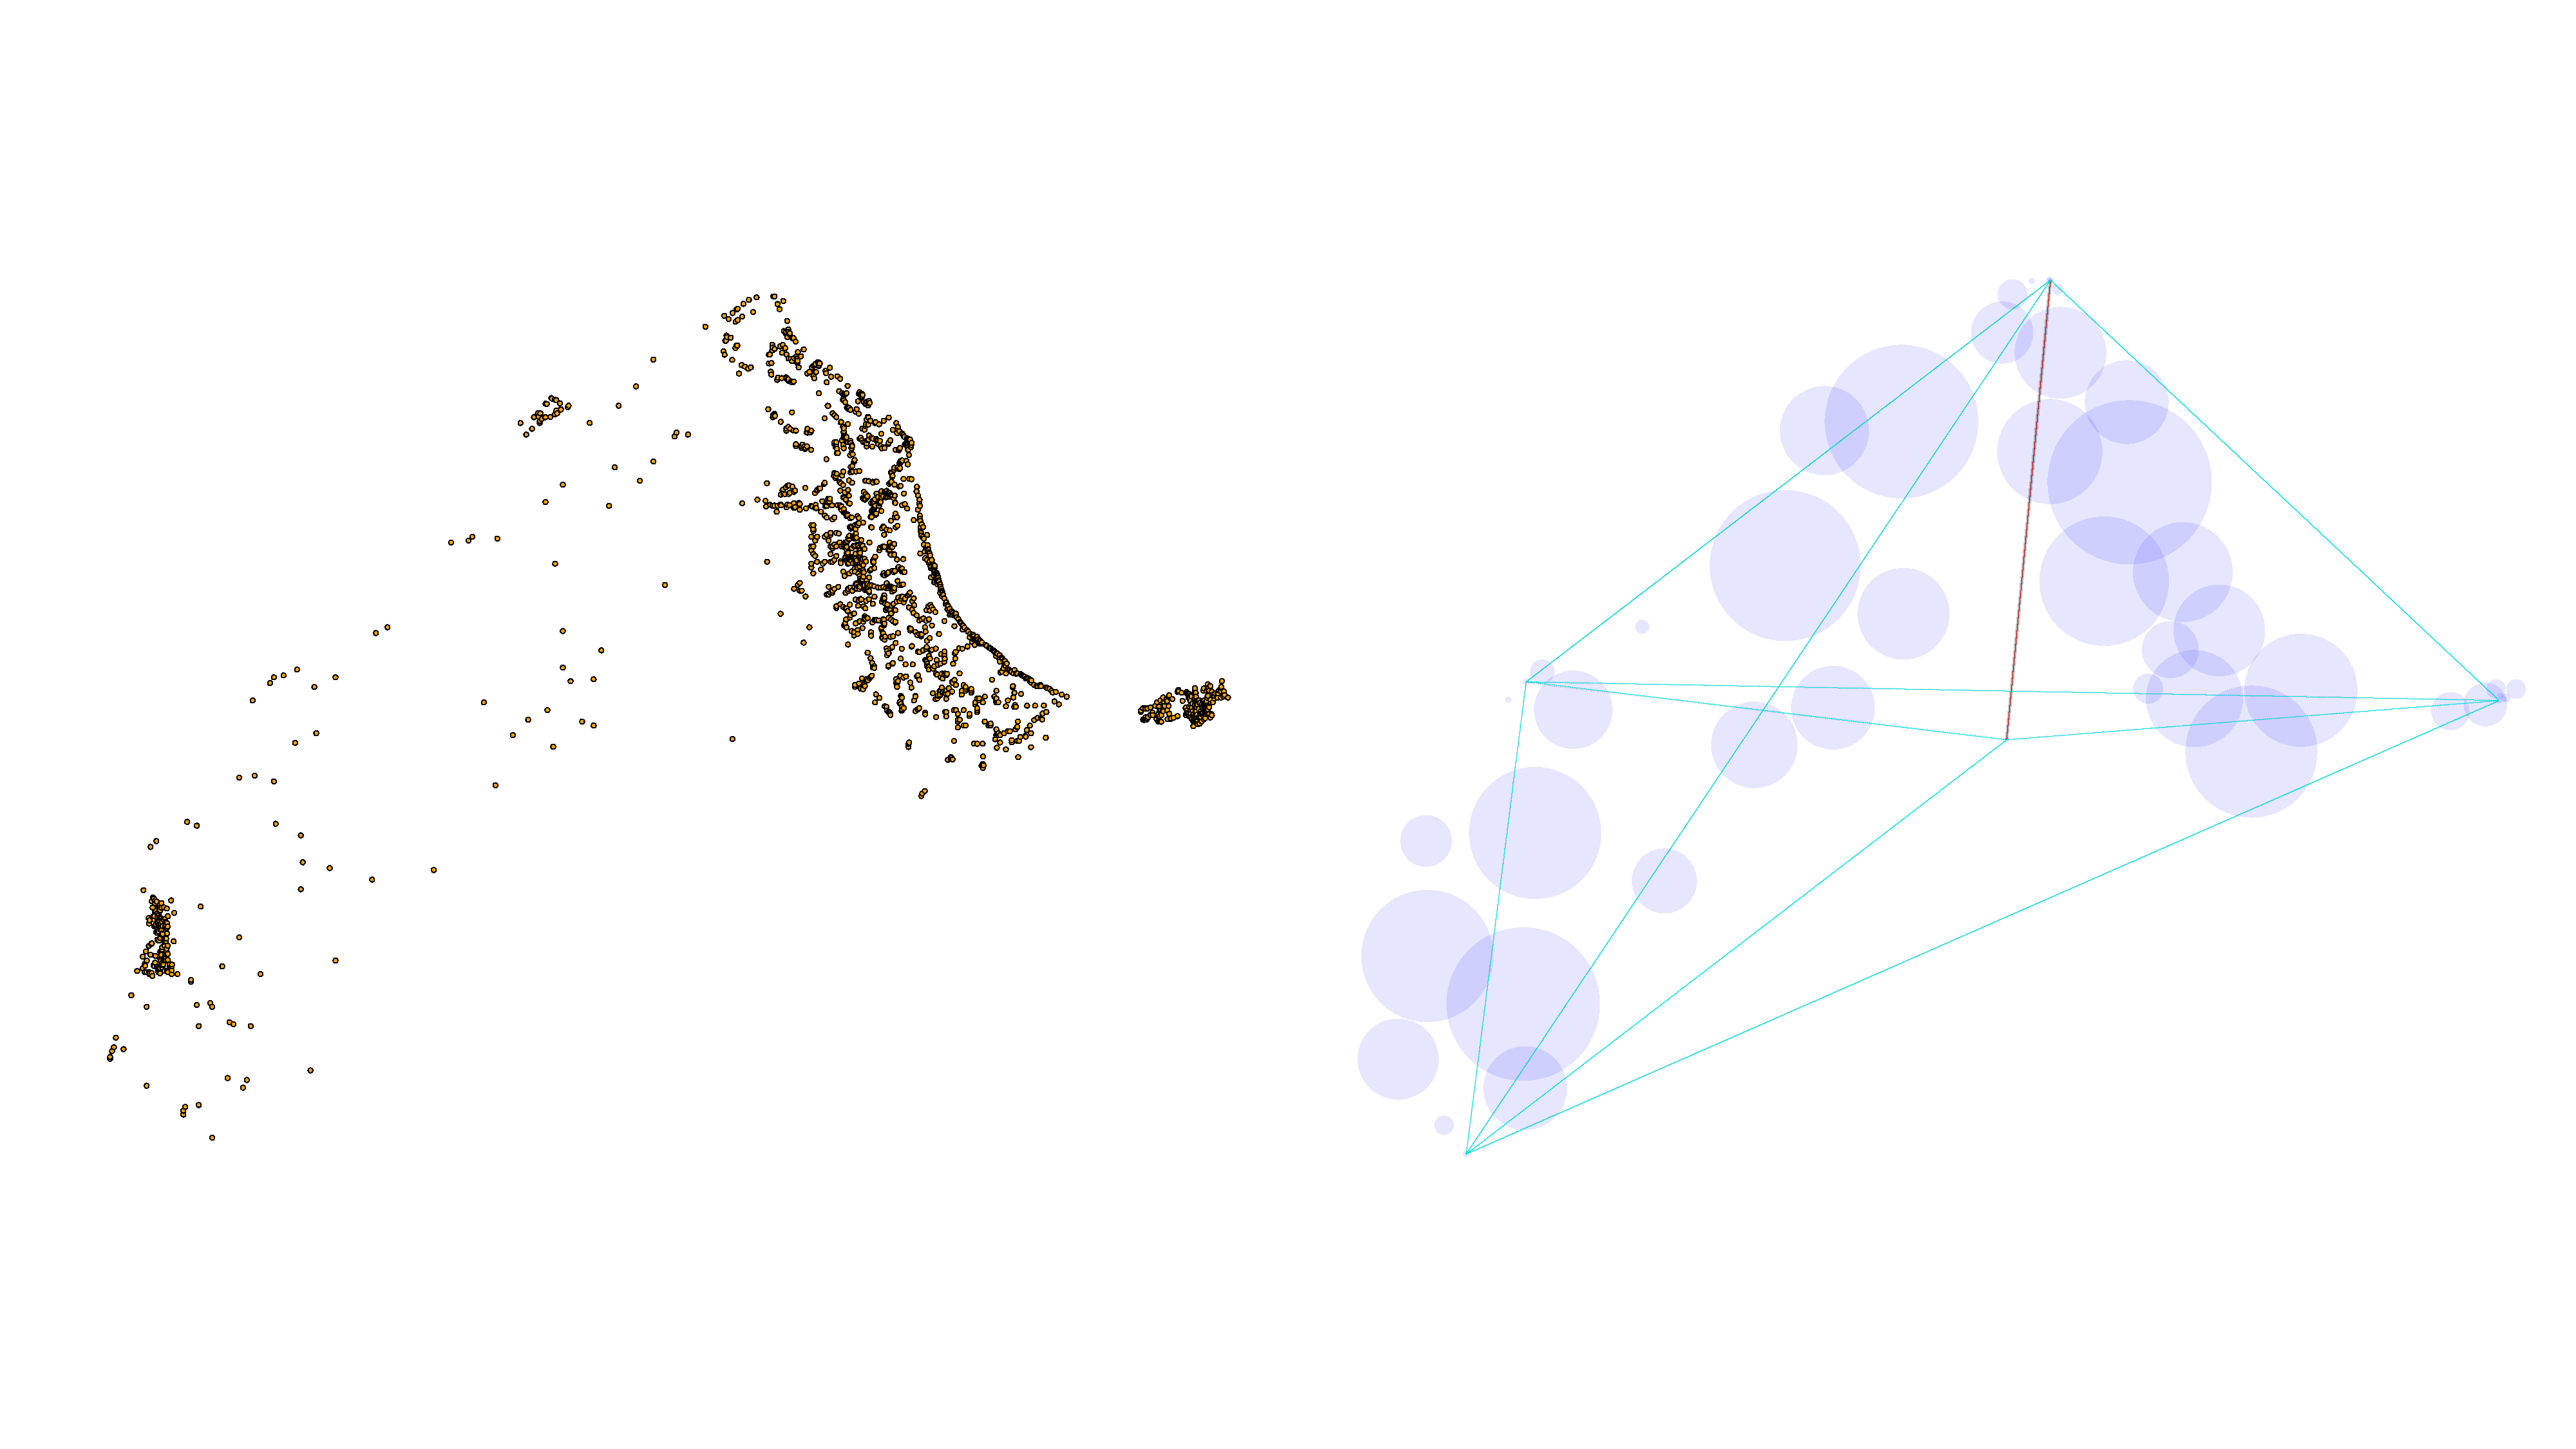
\includegraphics[width=16cm]{mu1979.pdf}
	\caption{Decremental clustering on instance \texttt{mu1979.tsp}\label{fig:mu1979} for $p = 5$}
\end{figure}

\subsection{Procedure \hpdp{D}{p}\label{section:decrclust:hpdp}}

In this section we describe a simple procedure to compute a non-trivial lower bound $L$ of problem \pdp{D}{p}. This procedure is far from producing a near-optimal solution to the problem, but is sufficient to feed the procedure \initclust{D}{p}{L} to be described later in Section \ref{section:decrclust:initclust}. We execute a $k$-means algorithm using the dissimlarity matrix $D$ to construct $p$ clusters. For each of the $p$ centers in the cluster, we find the node in each cluster that is closest to its center. Let us call this set of points $X = \{x_1\ldots x_p\}$. We compute $d\leftarrow \min\{D(x_i, x_j): 1\leq i < j \leq p\}$. This procedure is performed not once but multiple times for as long as the value $d$ keeps increasing. Indeed, we stop after 10 iterations without being able to improve this value. The highest possible such value $d$ is returned as lower bound $L$.

\subsection{Procedure \initclust{D}{p}{L}\label{section:decrclust:initclust}}

In this section we describe a two-step procedure used to build an initial sufficiently refined clustering of the $n$ points, using the lower bound $L$ as stopping point. In the first step, a $p$-clustering of the nodes is found using a $k$-means algorithm. This clustering may not be sufficiently refined and thus the second step is executed. This second step is iterative and goes as follows. At any given iteration ---say when the number of clusters has reached a value of $m$---, we check if the sizes of each cluster are strictly lower than $L$. If yes, the current clustering $\mC$ and dissimlarity matrix $\DmC$ are returned. Otherwise, we compute $i^*\leftarrow\arg\max\{\DmC(i, i): i = 1\ldots m\}$ and execute a $k$-means algorithm to further divide cluster $C_{i^*}$ into two clusters. The dissimilarity matrix $\DmC$ is then extended to dimensions $(m + 1)\times (m + 1)$. At this point, only the new rows and columns need to be recomputed to alleviate the computational effort.

\subsection{Procedure \splitadd{S}{W}{\mC}{\DmC}\label{section:decrclust:splitadd}}

In this section we describe a procedure that, given a clustering $\mC$, a dissmilarity matrix $\DmC$, a family $S$ of cluster indices with $|C_i|\geq 2$ for every $i\in S$ and a set of optimal cluster locations $W$ (with $S\subseteq W$), selects one cluster from those indexed in $S$ and splits it into two separate clusters. The extended clustering and dissimilarity matrix are returned. We first compute $(s^*, w^*)\leftarrow\arg\min\{\DmC(s, w), s\in S, w\in W\}$, which is the pair of indices in $S\times W$ with minimum dissimilarity. This computation excludes on purpose the pairs with both indices in $W\setminus S$ as both associated nodes are ---by construction of set $S$--- singletons. If $w^*\in S$, then for the following, the index with highest value of $\DmC(u, u)$ is kept, with $u \in \{s^*, w^*\}$. For the retained index, we execute a $k$-means algorithm similar to the one described in the previous section, to split the associated cluster into two separate clusters. We update and return the clustering $\mC$ and the dissimilarity matrix $\DmC$ accordingly.

\subsection{Procedure \solvePDP{\DmC}{p}\label{section:decrclust:solvepdp}}

In this section we introduce a heuristic and an exact solver for problem \pdp{\DmC}{p}. Without loss of generality and to alleviate the reading, we will drop the superindex $\mC$ from the dissimilarity matrix. Therefore, we will simply denote $D$ to refer to it. It goes without saying that we always execute the heuristic solver before any attempt at executing the exact one.

\subsubsection{Exact solver}

Our exact solver uses the pure-integer formulation introduced by \citet{Sayah2017new} and solves it by branch-and-cut embedded within a double binary search method. This formulation uses $m$ binary variables ---one per row/column of the matrix $D$--- to represent the location decisions, and $\Delta$ binary variables $z$, where $\Delta$ is the number of different values appearing in the matrix $D$. We refer to \citet{Sayah2017new} for details of the model and the associated valid inequalities.

Within the decremental clustering scheme, we exploit the existence of a monotonically decreasing upper bound $U$ and exploit this further within a double binary search scheme, as follows. Let us denote by \exactPDP{D}{p}{L}{U} the solver of problem \pdp{D}{p} when feeded with the additional lower and upper bounds $L$ and $U$. These bounds can be exploited in two aspects. First, to reduce the number of binary variables $z$. Second, to derive cutting planes to strengthen the model. The details of these two accelerating features can be found in full extent in \citet{Sayah2017new}. Our double binary search method starts with making $l, u \leftarrow U$. It iterates by executing \exactPDP{D}{p}{l}{u} at every iteration. If no feasible solution exists, the quantities are updated according to the formulas $l\leftarrow l - 2^t, u \leftarrow l - 1$, where $t$ is the iteration number. The problem \exactPDP{D}{p}{l}{u} is likely to be infeasible for a few iterations. We abort this procedure as soon as one feasible solution is identified and its objective value is used to update the lower bound. At this point, the final quantities $l, u$ are used to feed another binary search method with the aim of closing the gap between $l$ and $u$. For as long as $u > l$, we make $r\leftarrow \lceil (l + u) / 2\rceil$ and execute \exactPDP{D}{p}{r}{u}. If the problem is feasible, we make $l\leftarrow r$, otherwise we make $u\leftarrow r - 1$ and repeat.

\subsubsection{Heuristic solver}

We have observed that, in a large number of iterations, the optimal value of problem \pdp{D}{p} does not decrease from one iteration to the next. This type of degeneracy is often observed in decremental relaxation schemes \citep{Aloise2018sampling, Contardo2019scalable}. Therefore, before resorting to executing the exact solver described in the previous section, our heuristic scheme checks if it is possible to select $p$ points out of the $p + 1$ points identified from the previous iteration ---which includes $p - 1$ optimal clusters that remain untouched, plus the one that has been split into two--- as described in Section \ref{section:decrclust:splitadd}. If the value of this solution equals the upper bound $U$ from the last iteration, the associated solution is then optimal and there is no need to execute the exact solver.

\section{Computational experience\label{section:computation}}

In this section we provide computational evidence of the effectiveness of the proposed method. Our method has been coded in Julia v1.1 using the JuMP interface v18.5 with Gurobi v8.1 as multipurpose optimization solver. It runs on an Intel Xeon E5-2637 v2 @ 3.50 GHz with 128 GB of RAM. Although this machine is capable of executing code in parallel, for reproducibility purposes we limit the number of threads to one. We consider instances from the TSPLIB containing between 1,621 and 104,815 points in the euclidean plane. The dissimilarity between two points is computed according to the TSPLIB standard and considers only integral distances. We noticed that in some instances there exist points with identical coordinates. We proceed to remove all the redundant entries from an instance before beginning the optimization.

For each instance in the dataset, we consider four values of $p$, namely $p\in\{5, 10, 15, 20\}$. In addition to the algorithm described in this paper, we have also implemented a variant of \citet{Sayah2017new}'s algorithm embedded within the same double binary search method described in Section \ref{section:decrclust:solvepdp}. Using the notation described in our paper, this method resorts to executing procedure \solvePDP{D}{p} at once. We have executed both algorithms and given them a maximum CPU time of 86,400 seconds (1 day). Our implementation of \citeauthor{Sayah2017new}'s method could not handle problems containing 3,000 nodes or more (it rapidly ran out of memory), so the comparison between both methods is restricted to the smaller ones.

In Table \ref{table:small} we report a comparison between our method and our implementation of \citeauthor{Sayah2017new}'s method, restricted to the problems containing strictly less than 3,000 nodes. We report, for each method and for each value of $p$, the final upper bounds (under column labeled \texttt{UB}) and the elapsed CPU times in seconds (under column labeled \texttt{CPU}). We highlight in bold characters the upper bounds that match a proven optimal value. As the results show, our method is more robust and is capable of solving to proven optimality all the problems in this restricted testbed, something that our implementation of \citeauthor{Sayah2017new}'s method did not. For the problems solved by both methods, ours is always substantially faster.

\begin{table}[!hbtp]
	\centering
	\scalebox{0.6}{
		\begin{tabular}{|l|rr|rr|rr|rr|rr|rr|rr|rr|}
			\hline
			\multirow{3}{*}{Instance}& \multicolumn{8}{|c|}{\citet{Sayah2017new}}& \multicolumn{8}{|c|}{This paper}\\
			\cline{2-17}
			& \multicolumn{2}{|c|}{$p = 5$} & \multicolumn{2}{|c|}{$p = 10$} & \multicolumn{2}{|c|}{$p = 15$} & \multicolumn{2}{|c|}{$p = 20$} & \multicolumn{2}{|c|}{$p = 5$} & \multicolumn{2}{|c|}{$p = 10$} & \multicolumn{2}{|c|}{$p = 15$} & \multicolumn{2}{|c|}{$p = 20$}\\
			\cline{2-17}
			& UB & CPU & UB & CPU & UB & CPU & UB & CPU & UB & CPU & UB & CPU & UB & CPU & UB & CPU\\
			\hline
			\texttt{rw1621.tsp} & \textbf{971} & 206.8 & \textbf{558} & 163.2 & \textbf{407} & 474.9 & \textbf{339} & 582.8 & \textbf{971} & 16.1 & \textbf{558} & 17.8 & \textbf{407} & 24.4 & \textbf{339} & 32.2\\
			\texttt{u1817.tsp} & \textbf{1,535} & 690.6 & \textbf{881} & 1,897.4 & \textbf{665} & 7,046.3 & 1,077 & TL & \textbf{1,535} & 27.6 & \textbf{881} & 52.6 & \textbf{665} & 371.9 & \textbf{559} & 1,578.9\\
			\texttt{rl1889.tsp} & \textbf{10,166} & 4,475.0 & \textbf{5,846} & 3,630.3 & \textbf{4,478} & 72,237.8 & 4,706 & TL & \textbf{10,166} & 28.6 & \textbf{5,846} & 74.8 & \textbf{4,478} & 221.3 & \textbf{3,727} & 400.3\\
			\texttt{mu1979.tsp} & \textbf{3,845} & 1,327.9 & \textbf{2,159} & 1,100.2 & \textbf{1,562} & 1,781.7 & \textbf{1,229} & 2,085.2 & \textbf{3,845} & 28.2 & \textbf{2,159} & 30.7 & \textbf{1,562} & 33.3 & \textbf{1,229} & 63.4\\
			\texttt{pr2392.tsp} & \textbf{8,086} & 9,830.1 & \textbf{4,976} & 18,112.0 & \textbf{3,788} & 73,647.6 & 3,173 & TL & \textbf{8,086} & 38.7 & \textbf{4,976} & 121.9 & \textbf{3,788} & 375.0 & \textbf{3,150} & 6,990.6\\
			\texttt{d15112-modif-2500.tsp} & \textbf{12,217} & 24,402.8 & \textbf{7,132} & 22,290.7 & \textbf{5,771} & 12,580.9 & 4,776 & TL & \textbf{12,217} & 46.1 & \textbf{7,132} & 95.9 & \textbf{5,771} & 222.8 & \textbf{4,773} & 583.7\\
			\hline
	\end{tabular}}
	\caption{Method comparison on small instances\label{table:small}}
\end{table}


In Table \ref{table:large} we report the results obtained by our method for the problems containing 3,000 or more nodes. We report, for each value of $p$, the final upper bound (under column labeled \texttt{UB}), the CPU time in seconds (under column labeled \texttt{CPU}), and the final number of clusters at the final iteration (under column labeled \texttt{C}). Once again, we mark in bold characters whenever a problem is solved to proven optimality. In the last two rows we report ---for each value of $p$--- the total number of problems solved to proven optimality as well as the average CPU times and the average number of clusters restricted to the problems solved to proven optimality. As the results show, our method is robust for solving \pDP{}s for small values of $p$. Only one in 68 problems could not be solved within the time limit of one day for $p\leq 10$. For larger values of $p$, the method is less robust but still capable of handling some very large problems. We would like to remark that the largest instance considered in this study, namely problem \texttt{sra104815.tsp} would require more than 40 GB of RAM if the full dissimilarity matrix had to be stored in RAM, let alone to load and solve the associated integer program required to execute \citeauthor{Sayah2017new}'s method. Our method avoids this storage and never required more than 2 GB to run even for the largest problems.

\begin{table}[!hbtp]
	\centering
	\scalebox{0.79}{
		\begin{tabular}{|l|rrr|rrr|rrr|rrr|}
			\hline
			\multirow{2}{*}{Instance} & \multicolumn{3}{|c|}{$p = 5$} & \multicolumn{3}{|c|}{$p = 10$} & \multicolumn{3}{|c|}{$p = 15$} & \multicolumn{3}{|c|}{$p = 20$}\\
			\cline{2-13}
			& \texttt{UB} & \texttt{CPU} & \texttt{C} & \texttt{UB} & \texttt{CPU} & \texttt{C} & \texttt{UB} & \texttt{CPU} & \texttt{C} & \texttt{UB} & \texttt{CPU} & \texttt{C}\\
			\hline
			\texttt{pcb3038.tsp} & \textbf{2,390} & 49.8 & 65 & \textbf{1,414} & 478.1 & 452 & \textbf{1,075} & 4,275.8 & 781 & \textbf{898} & 15,851.1 & 1050\\
			\texttt{nu3496.tsp} & \textbf{2,462} & 33.8 & 59 & \textbf{1,524} & 47.2 & 161 & \textbf{1,092} & 91.6 & 334 & \textbf{926} & 105.8 & 410\\
			\texttt{ca4663.tsp} & \textbf{34,256} & 97.1 & 71 & \textbf{20,267} & 142.8 & 227 & \textbf{15,467} & 165.8 & 276 & \textbf{12,376} & 208.3 & 357\\
			\texttt{rl5915.tsp} & \textbf{9,793} & 166.9 & 108 & \textbf{6,160} & 217.5 & 234 & \textbf{4,544} & 14,236.0 & 1024 & \textbf{3,887} & 16,894.9 & 987\\
			\texttt{rl5934.tsp} & \textbf{10,396} & 171.9 & 110 & \textbf{5,951} & 713.7 & 454 & \textbf{4,576} & 3,904.0 & 762 & \textbf{3,817} & 25,333.0 & 1096\\
			\texttt{tz6117.tsp} & \textbf{6,116} & 207.8 & 157 & \textbf{3,818} & 249.7 & 307 & \textbf{2,887} & 1,100.9 & 619 & \textbf{2,401} & 3,190.1 & 828\\
			\texttt{eg7146.tsp} & \textbf{5,247} & 236.4 & 83 & \textbf{3,187} & 265.0 & 172 & \textbf{2,377} & 264.0 & 213 & \textbf{1,833} & 433.0 & 390\\
			\texttt{pla7397.tsp} & \textbf{374,026} & 273.3 & 78 & \textbf{238,412} & 342.5 & 229 & \textbf{183,522} & 544.8 & 420 & \textbf{148,000} & 1,218.7 & 654\\
			\texttt{ym7663.tsp} & \textbf{4,974} & 242.0 & 71 & \textbf{2,743} & 274.1 & 143 & \textbf{1,987} & 332.8 & 292 & \textbf{1,578} & 723.3 & 554\\
			\texttt{pm8079.tsp} & \textbf{2,078} & 113.3 & 60 & \textbf{1,347} & 121.0 & 167 & \textbf{941} & 157.0 & 309 & \textbf{805} & 168.1 & 417\\
			\texttt{ei8246.tsp} & \textbf{2,426} & 308.1 & 118 & \textbf{1,500} & 361.9 & 311 & \textbf{1,113} & 3,542.0 & 863 & \textbf{939} & 12,292.2 & 1156\\
			\texttt{ar9152.tsp} & \textbf{13,820} & 173.0 & 57 & \textbf{8,117} & 239.4 & 216 & \textbf{6,371} & 429.9 & 422 & \textbf{5,019} & 5,184.0 & 833\\
			\texttt{ja9847.tsp} & \textbf{10,651} & 352.6 & 69 & \textbf{5,405} & 393.8 & 153 & \textbf{3,907} & 436.7 & 198 & \textbf{3,055} & 531.0 & 441\\
			\texttt{gr9882.tsp} & \textbf{4,295} & 432.6 & 113 & \textbf{2,633} & 501.3 & 274 & \textbf{1,969} & 616.8 & 443 & \textbf{1,625} & 677.4 & 525\\
			\texttt{kz9976.tsp} & \textbf{13,969} & 415.9 & 94 & \textbf{8,607} & 495.5 & 285 & \textbf{6,360} & 835.2 & 479 & \textbf{5,230} & 5,189.4 & 937\\
			\texttt{fi10639.tsp} & \textbf{6,284} & 479.3 & 83 & \textbf{3,767} & 704.6 & 407 & \textbf{2,806} & 2,588.7 & 716 & \textbf{2,322} & 17,955.2 & 1146\\
			\texttt{rl11849.tsp} & \textbf{10,736} & 556.3 & 91 & \textbf{6,243} & 1,065.9 & 477 & \textbf{4,719} & 7,836.8 & 908 & \textbf{4,000} & 32,583.2 & 1214\\
			\texttt{usa13509.tsp} & \textbf{229,767} & 712.3 & 66 & \textbf{133,500} & 1,082.1 & 330 & \textbf{99,689} & 7,022.5 & 726 & 83,538 & TL & 1413\\
			\texttt{brd14051.tsp} & \textbf{4,379} & 694.7 & 68 & \textbf{2,465} & 1,161.8 & 358 & \textbf{1,862} & 2,025.2 & 681 & \textbf{1,569} & 4,317.6 & 872\\
			\texttt{mo14185.tsp} & \textbf{4,748} & 784.8 & 76 & \textbf{2,803} & 949.9 & 299 & \textbf{2,125} & 1,785.6 & 641 & \textbf{1,746} & 5,526.7 & 960\\
			\texttt{ho14473.tsp} & \textbf{2,357} & 215.5 & 75 & \textbf{1,427} & 315.0 & 274 & \textbf{1,104} & 429.0 & 452 & \textbf{914} & 5,563.1 & 934\\
			\texttt{d15112.tsp} & \textbf{12,348} & 1,127.7 & 168 & \textbf{7,319} & 4,003.8 & 704 & \textbf{5,907} & 9,635.4 & 932 & \textbf{4,944} & 84,652.7 & 1384\\
			\texttt{it16862.tsp} & \textbf{5,855} & 1,187.3 & 98 & \textbf{3,407} & 1,246.1 & 171 & \textbf{2,468} & 1,572.3 & 425 & \textbf{2,100} & 1,870.6 & 610\\
			\texttt{d18512.tsp} & \textbf{4,396} & 1,570.8 & 164 & \textbf{2,599} & 4,752.5 & 801 & \textbf{2,109} & 10,771.2 & 1050 & \textbf{1,762} & 38,044.8 & 1269\\
			\texttt{vm22775.tsp} & \textbf{5,348} & 1,708.1 & 72 & \textbf{2,789} & 2,134.8 & 177 & \textbf{2,237} & 2,676.0 & 386 & \textbf{1,817} & 2,934.2 & 612\\
			\texttt{sw24978.tsp} & \textbf{7,128} & 2,181.0 & 81 & \textbf{4,196} & 3,030.5 & 348 & \textbf{3,149} & 4,869.8 & 714 & \textbf{2,681} & 20,742.0 & 1276\\
			\texttt{fyg28534.tsp} & \textbf{565} & 3,374.2 & 91 & \textbf{340} & 35,256.4 & 1314 & \textbf{276} & 12,926.6 & 1131 & 230 & TL & 1556\\
			\texttt{bm33708.tsp} & \textbf{7,094} & 4,195.4 & 116 & \textbf{3,867} & 5,662.3 & 235 & \textbf{2,876} & 16,009.8 & 1113 & \textbf{2,390} & 23,630.3 & 1229\\
			\texttt{pla33810.tsp} & \textbf{417,437} & 5,544.0 & 164 & \textbf{262,557} & 44,046.0 & 833 & 207,885 & TL & 1017 & 178,213 & TL & 860\\
			\texttt{bby34656.tsp} & \textbf{623} & 4,639.8 & 92 & \textbf{377} & 10,758.9 & 861 & \textbf{299} & 23,676.6 & 1268 & 251 & TL & 1488\\
			\texttt{pba38478.tsp} & \textbf{698} & 6,203.4 & 94 & \textbf{407} & 9,829.3 & 669 & \textbf{311} & 38,457.8 & 1464 & 266 & TL & 1596\\
			\texttt{ch71009.tsp} & \textbf{22,263} & 21,811.4 & 117 & \textbf{14,353} & 25,522.2 & 547 & \textbf{10,845} & 38,990.8 & 1011 & \textbf{9,311} & 38,499.4 & 1221\\
			\texttt{pla85900.tsp} & \textbf{553,829} & 32,147.4 & 161 & 348,661 & TL & 843 & 278,770 & TL & 807 & 240,465 & TL & 705\\
			\texttt{sra104815.tsp} & \textbf{1,066} & 52,593.4 & 200 & \textbf{669} & 64,275.4 & 567 & \textbf{518} & 76,409.9 & 1113 & 432 & TL & 1332\\
			\hline
			Optimal & \multicolumn{3}{|c|}{34/34} & \multicolumn{3}{|c|}{33/34} & \multicolumn{3}{|c|}{32/34} & \multicolumn{3}{|c|}{27/34}\\
			Average & & 4,265 & 100 & & 6,686 & 399 & & 9,019 & 693 & & 13,493 & 865\\
			\hline
	\end{tabular}}
	\caption{Decremental clustering on large instances\label{table:large}}
\end{table}

\section{Concluding remarks\label{section:conclusions}}

We have introduced a decremental clustering method for the solution of the $p$-dispersion problem (\pDP{}). Our method works by building an initial clustering of the nodes and by refining this clustering in an iterative fashion. In each iteration, a restricted \pDP{} is solved to compute upper bounds of the problem. In practice, for small values of $p$, we are capable of proving optimality within a few iterations for problems containing up to 100,000 nodes, this is orders of magnitude larger than the limits of previous methods. To the best of our knowledge, this is the first time that a clustering technique is embedded within an exact solver for location analysis. As an avenue of further research, we believe that the algorithm could be adapted to solve variants of the \pDP{} or other location problems with a potential to benefit from clustering techniques. While this potential is well understood in the scientific literature on non-supervised learning and heuristics for combinatorial optimization, their use within exact methods is rather new and its full potential is yet to be understood in more depth.

\section*{Acknowledgments}

The author thanks the Natural Sciences and Engineering Research Council of Canada (NSERC) under Discovery Grant 435824-2013 for its financial support.

\bibliographystyle{informs2014}
\bibliography{refs}

\end{document}





